\subsection{Overview}
An essential part of the platform design is to satisfy not only functional requirements but non-functional requirements as well.This means that architectural choices are crucial at this point of the development for the sake of achieving the desired output in terms of requirements ,performance ,scalability and user experience.\\
An important focus will be set on how the different systems interact with each other and the back-end to obtain the events as required by sec. 3 of the RASD.Furthermore choices regarding up scaling and redundancy will be discussed.\\

%----------------%
% COMPONENT VIEW %
%----------------%
\subsection{Component View}
This section focuses on the component overview giving an insight on their core functionality and various interfaces.For more detailed information about component interfaces see \hyperref[sec:CInter]{\emph{section 2.5}} \\
A first classification of components can be made at a high level:
\begin{itemize}
\item \textbf{\hyperref[sec:Server]Server} provides the core functionality of the platform. The server incorporates the biggest part of the \emph{business logic} and stores some \emph{data} locally.
\item \textbf{\hyperref[sec:UserClient]User Client} provides a high level representation of the real user clients. It is considered a \emph{thin client} as it leaves most of the functionalities to the Server.
\item \textbf{\hyperref[sec:OnBClient]On-Board Client} provides navigation functionalities done exclusively client-side , whilst other functionalities are left to the server side (like  authentication).
\end{itemize}
As mentioned above the platform is designed using the \emph{client-server}paradigm. Component interactions are handled by the server which is able to receive calls from the clients . Client interaction is never done peer to peer but via server.


\subsubsection{Server}
The server is composed of :\\[0.4in]
\textbf{Back-End Application}\\[0.1in]
The Back-End Application is the  component that handles most of the business logic.
The application is written in Java EE and to fulfil its tasks (see section
3 of the RASD) it needs to interface with the Internet network using
the HTTPS protocol and the JAVA API for RESTful Web Service, with a
MySQL database and GooleMaps API.\\[0.4in]
\textbf{Back-End internal components}\\[0.1in]
\begin{itemize}

\item \textbf{User manager}\\
This component handles user data, registration and authentication.The user manager has direct access to the DBMS and receives read and write requests from the RESTful API.

\item \textbf{Notification manager}\\
This component is responsible for implementing the push notification service towards
the user-side applications.
It is necessary to have this type of module running in the back-end because
there are cases in which a communication must happen between the clients and
the back-end, but no direct request is made to the RESTful API by the clients:
for example when the reserved car is nearby, the system must send the user a 'ready to unlock' notification.

\item \textbf{Vehicle manager}\\
The car manager component's job is to manage all the vehicles throughout the city.It can access the DBMS to query vehicle information but stores essential vehicle information locally such as location ,battery level and number of seats.Car positions
are managed through the Position manager.

\item \textbf{Position manager}\\
Keeps track of car positions around the city. When the Search manager gets triggered it forwards requests to the Position manager to get all available cars in compliance to the user input. It updates car positions through the vehicle manager at the end of each ride through the Vehicle manager. Moreover it handles the fair car distribution scenario when triggered by the on-board display. 

\item \textbf{Search manager}\\
The search manager component handles all incoming search requests forwarded by the user applications and interfaced through the RESTful API. The main functionality is to handle the user input and query the vehicle manager accordingly, returning the desired output to the user.\\In the event of a booking request the search manager forwards the demand to the Ride Manager.

\item \textbf{Ride manager}\\
The Ride manager component examines all incoming reservation request and creates \textit{Ride objects} according to the user selection and user data.The ride manager
is connected to the following components:
\begin{itemize}
\item \textit{Vehicle manager}: need to communicate and receive communications about car status changes in terms of availability, battery level and location.
\item \textit{Notification manager}: need to inform the user about remaining time to unlock the car or send the user 'ready to unlock ' notifications. Moreover it sends messages to the on-board display to inform the user about the response to a \textit{end ride request}.\\[0.4in] 
\end{itemize}
 
\end{itemize}

\textbf{Data Base}\\[0.1in]
The MySQL database fulfills the task of storing and granting access to all
the data generated and used by the service.\\
The connection between the Java EE application and the Data Base is supported
by the \emph{JDBC connector} \footnote{\url{http://dev.mysql.com/downloads/connector/j/}}.For more information about the data base see \hyperref[sec:DMV]{\emph{section 2.7}}.


\subsubsection{User Client}

As stated in section 2.4.2 of the RASD a native mobile application is developed
for Android, iOS and Windows Phone as well as Web application for the main browsers.
To fulfil the requirements expressed in section 3 of the
RASD, all the clients need to communicate with the Server making calls to
the REST API using platform specific API for REST HTTP calls.

\subsubsection{On-Board Client}
The on-board client needs to provide navigation functionality without interacting with the PowerEnjoy Server but directly through GoogleMaps API. At the beginning of each ride an authentication via PinCode is requested and verified server side.\\Safe Areas are stored locally on the client and updated only when the changes on the DB occur.On the other hand charging stations need to be updated in real-time as it can happen that charging stations are currently out of capacity.
\clearpage

\FloatBarrier
\begin{figure}
\subsubsection{Diagrams}
\centering
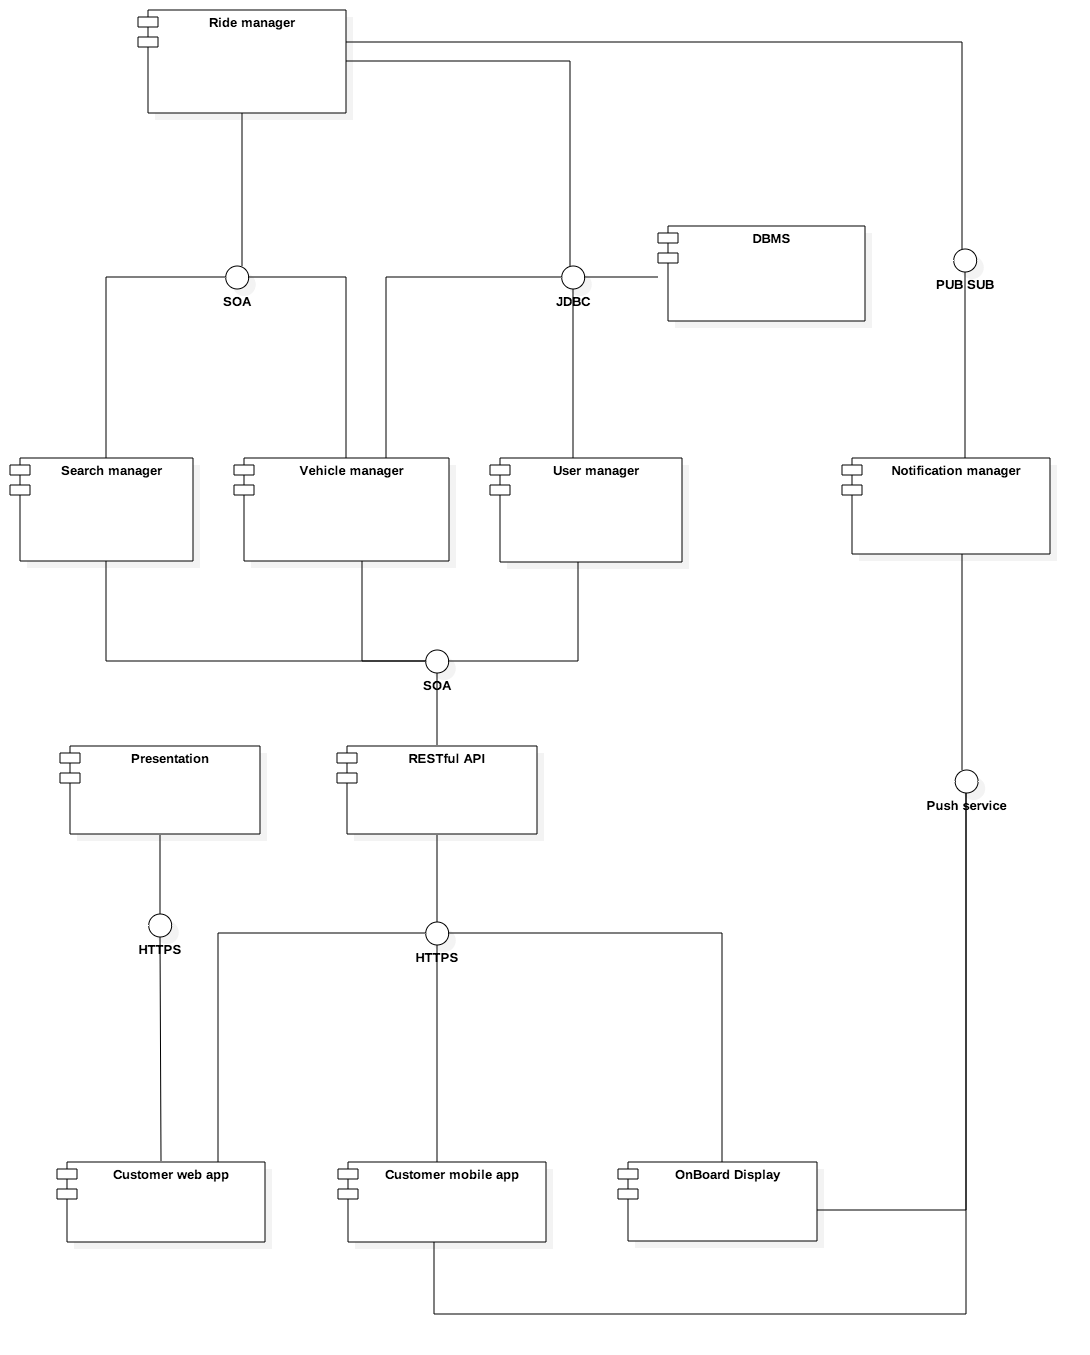
\includegraphics[scale=0.37]{Images/ComponentDiagram/ComponentDiagram.png}
\caption{Component Diagram}
\end{figure}
\FloatBarrier
\clearpage
\FloatBarrier
\begin{sidewaysfigure}
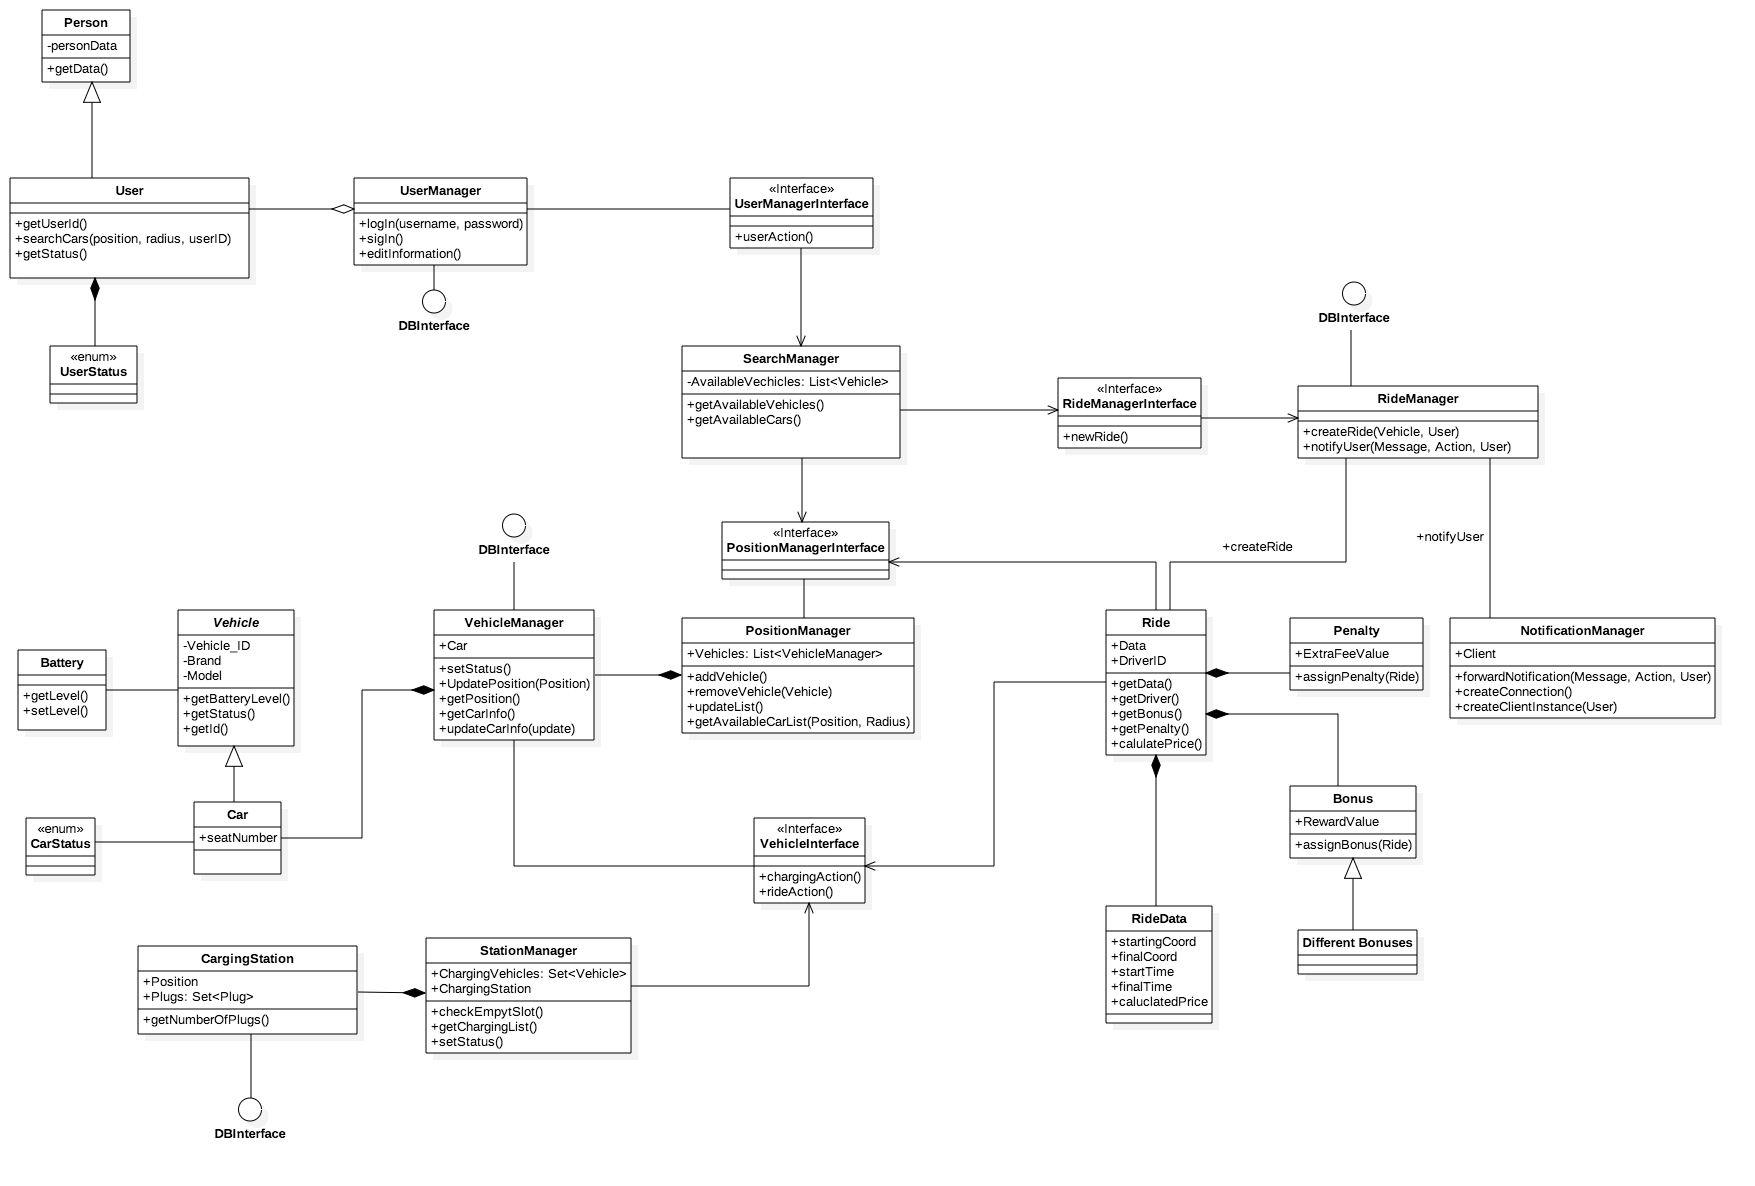
\includegraphics[scale=0.4]{Images/ClassDiagram/BackEnd.png}
\caption{Back-End Class Diagram}
\end{sidewaysfigure}
\FloatBarrier
\FloatBarrier
\begin{figure}
\hspace{-15mm}
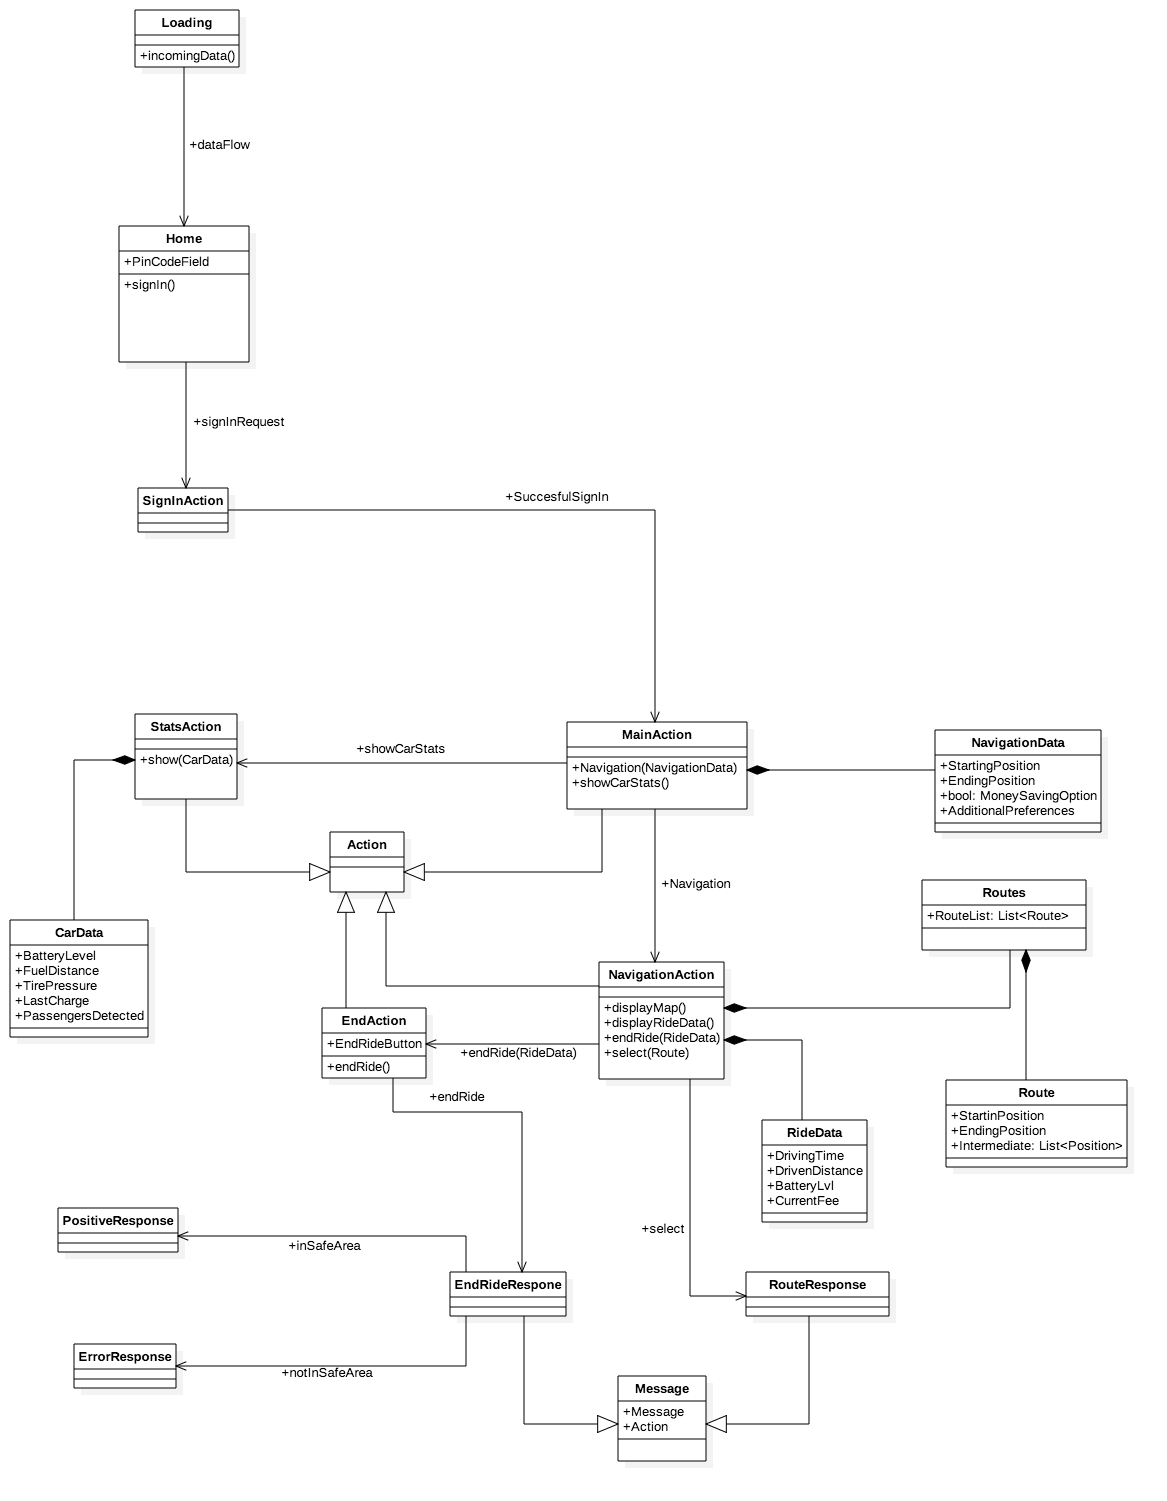
\includegraphics[scale=0.35]{Images/ClassDiagram/User.png}
\caption{User Application Class Diagram}
\end{figure}
\FloatBarrier
\FloatBarrier
\begin{figure}
\hspace{-15mm}
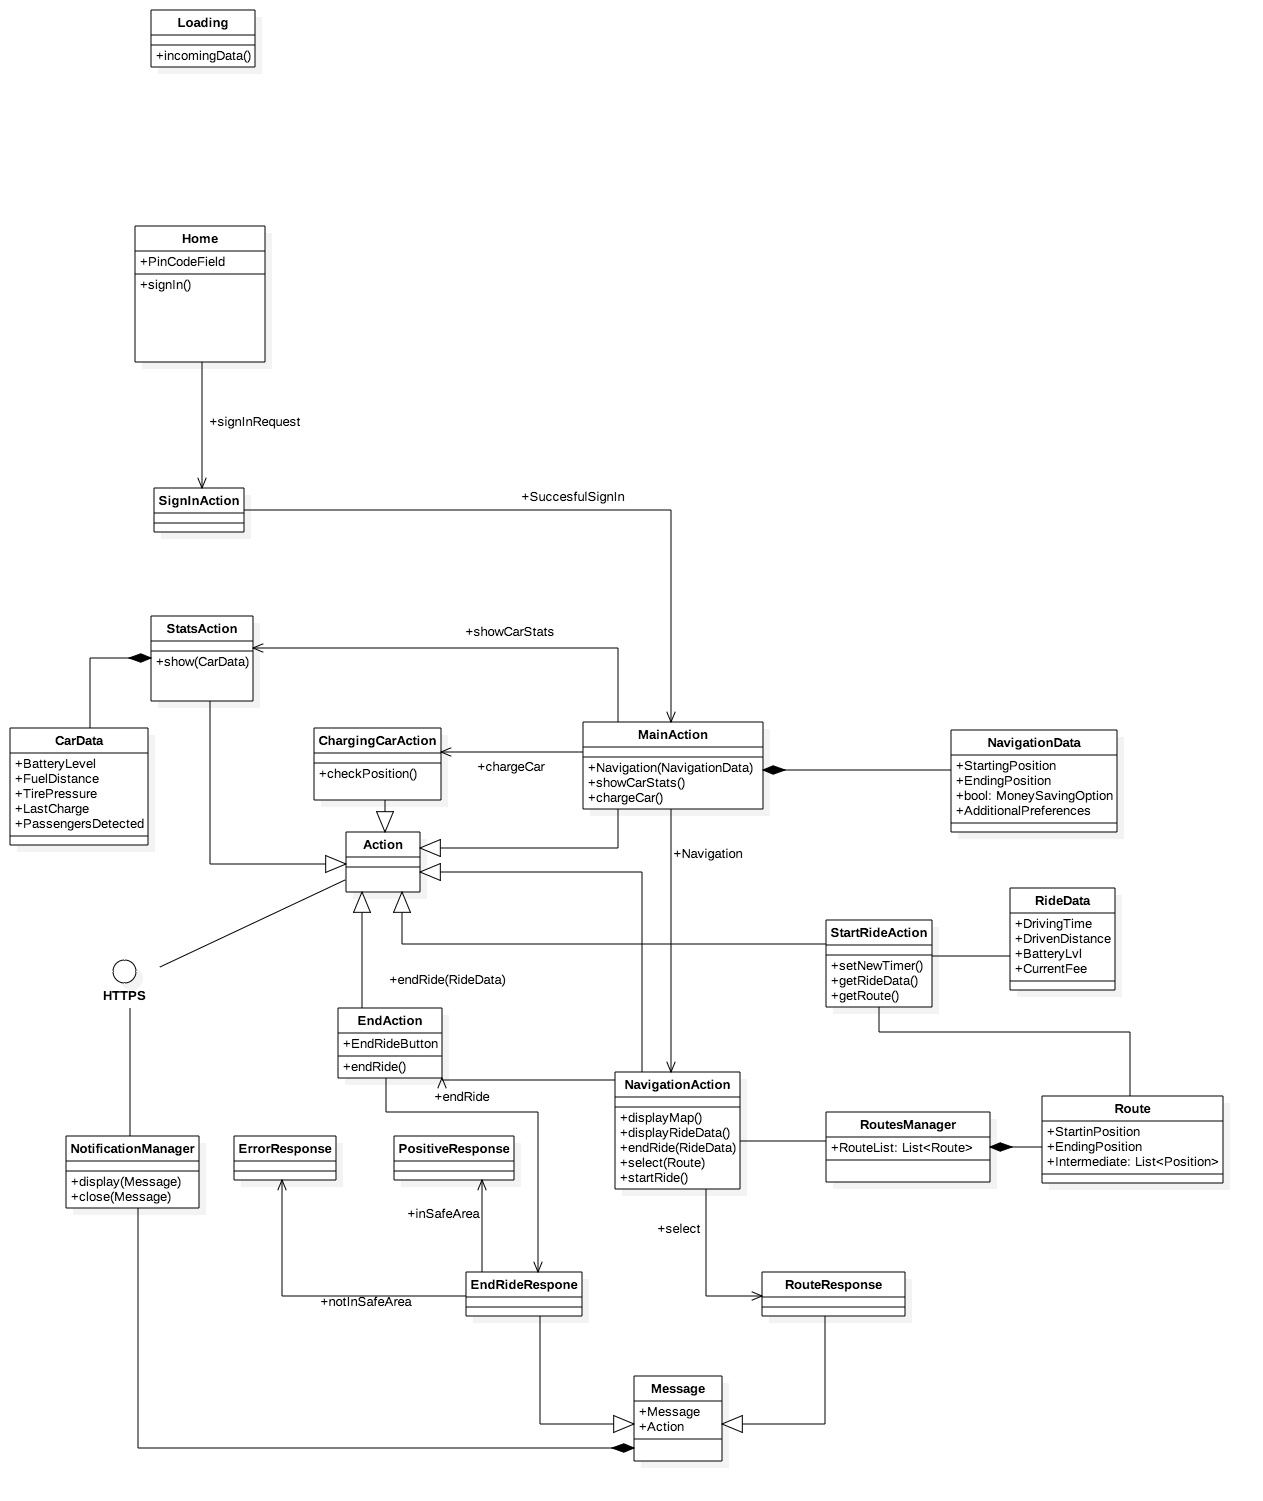
\includegraphics[scale=0.35]{Images/ClassDiagram/Display.png}
\caption{On-board Class Diagram}
\end{figure}
\FloatBarrier
\newpage

\subsection{Deployment View}
The following section contains a schema of the hardware infrastructure.
It was decided to omit the representation of the purely network-related hardware (routers, switches, etc.).
The chosen architecture is a typical web-based client-server architecture,
with the following components:
\begin{enumerate}
\item \textbf{Primary and BackUp Storage}: the Primary DB is a long term storage system on which the operational database is saved. This node provides the highest Read/Write speeds and is used in normal operational regime.The BackUP DB is a long term storage system with high reliability property. It is mainly used to store data backups and becomes fully operational in the event of total failure of the Primary RDBMS or DBMS nodes.
\item \textbf{Primary RDBMS Server}: server dedicated to run the DBMS software on account of the main server  and to manage the communication with the secondary storage node. This node is connected to the main server, from which it receives requests, and the storage nodes (either primary or secondary - the connection is transparent to the node and is hot-swappable in the event of a failure).
\item \textbf{Secondary RDBMS Server}:server dedicated to run the DBMS software and
manage the backup requests from the primary DBMS server. The node is connected to the secondary storage and to the primary DBMS server, for the reasons described above.
\item \textbf{Server}: a typical rack of servers dedicated to run the main back-end application.
\item \textbf{Web Server}:server dedicated to run the web server software and manage the load balancing towards the main server array. It is isolated by firewalls to  minimize the risk of unauthorized access to the main back-end components (especially to the storage nodes).
\item \textbf{User Application}:
\item \textbf{On-Board Display}:

\end{enumerate}

\FloatBarrier
\begin{figure}
\centering
\hspace{-5mm}
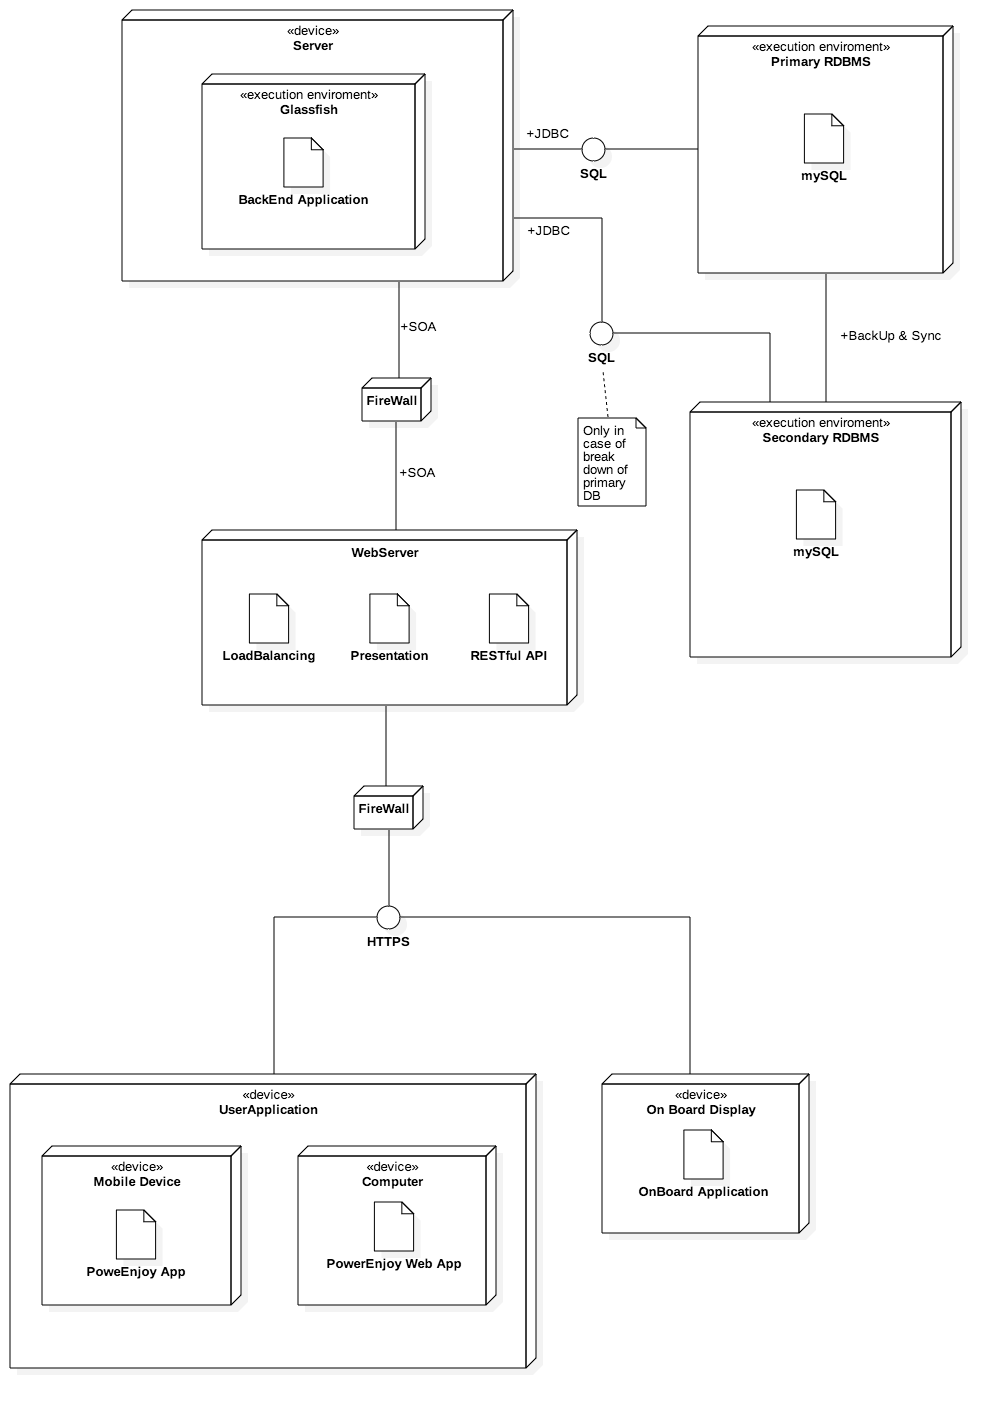
\includegraphics[scale=0.38]{Images/DeployDiagram/Deploy2.png}
\caption{Deployment Diagram}
\end{figure}
\FloatBarrier


\subsection{Runtime View}
\newpage


\subsection{Component Interfaces}
\label{sec:CInter}

\textbf{RESTful API}\\The RESTful API is a gateway communicator between clients and the back-end system: it's a stateless service which provides methods for data submission or requests returning the requested computations as a result.\\
RESTful API are an optimal solution for an application that must handle a vast number of users on a different number of platforms as it allows to guarantee the same user experience on all platforms. Furthermore the architectural properties positively affected by the constraints of the REST architectural include many important quality requirements such as performance, scalability and reliability.
\newpage
\subsection{Selected architectural styles and patterns}
\newpage

%----------------%
% DATA VIEW %
%----------------%
\subsection{Data Management view}
\label{sec:DMV}
This section focuses on how the data is stored and structured.
\subsubsection{Storing policy}
Data storage about people or physical belongings to PowerEnjoy are never automatically eliminated from the DB. On the other hand \emph{Rides} older than 2 years are automatically eliminated from the DB to save storage space and 
speed up search queries.\\
In order to reduce the load on the Server and to speed up user’s query
response, all the data that does not change frequently (like the user’s profile
data) is saved locally on the device and reloaded only when a modification
of the profile occurs.

\subsubsection{Entity-Relation Diagram}
\begin{center}
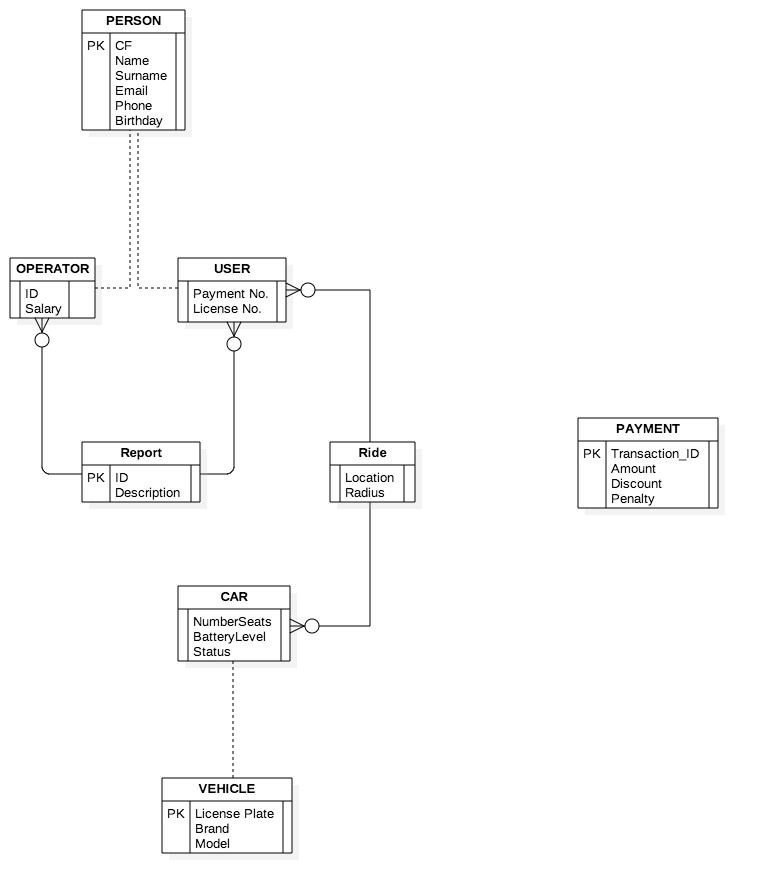
\includegraphics[scale=0.35]{Images/ER/ER.png}
\end{center}
The above shown figure represents the structure of the database. For better readability only vital entities are represented while others (like employees or managers) are omitted.
\begin{itemize}
\item \textit{Person}: is the generalisation of the operator and user entities. 
It holds common information and is identified by a \emph{Codice Fisicale}. All attributes must be different from null.
\item \textit{Operator}: is a person with a \emph{Salary} and an \emph{ID}. Operators can handle $0$ or more Reports.
\item \textit{User}: have an encoded \emph{password} and a valid \emph{license number} which must be provided together with other personal data during the registration process.The \emph{payment number} attribute can hold the null value initially. The \emph{PinCode} is a 4 digit number generated randomly during the registration process. Users can \emph{issue} reports ($0$ ore more) and can be drivers of cars ($0$ or more)
\item \textit{Report}: identified by an \emph{ID} and provided with a description attribute. Each report is associated with one Operator and one User.If the report is about a car it can hold a reference to said car ( \emph{hasIssue} has cardinality $0$,$1$).
\item \textit{Vehicle}: identified by a \emph{License Plate}. Each vehicle has also
a \emph{Brand} and \emph{Model} attribute.It is the generalisation of the \emph{Car} entity. A generalisation is useful as future implementations can include other means of transport.
\item \textit{Car}: \emph{status} holds a boolean value to show if the car is available or under maintenance.Available cars can be involved in \emph{Rides} or can be \emph{charging}.A car can be involved in $0$ or more rides , and can be listed in $0$ or more \emph{chargingCar } relations.
\item \textit{Charging Station}: identified by an \emph{ID}. Each charging station can be listed in $0$ or more \emph{chargingCars}relations.
\item \textit{Ride}: identified by an \emph{RideID}. Important attributes are \emph{Passenger No.} which determine eventual bonuses or penalties. Each Ride has exactly one car, one user and one payment.
\emph{Payment}: holds an \emph{Transaction ID} attribute as identifier.The amount, discount and penalty values are saved. The value of \emph{Amount} must be greater than $1$ , while the others greater than $0$. A payment is involved in exactly one ride.
\end{itemize}
\newpage